\documentclass[a4paper,11pt]{article}
\usepackage{amsmath,amsthm,amsfonts,amssymb,amscd,amstext,vmargin,graphics,graphicx,tabularx,multicol} 
\usepackage[francais]{babel}
\usepackage[utf8]{inputenc}  
\usepackage[T1]{fontenc} 
\usepackage{pstricks-add,tikz,tkz-tab,variations}
\usepackage[autolanguage,np]{numprint} 

\setmarginsrb{1.5cm}{0.5cm}{1cm}{0.5cm}{0cm}{0cm}{0cm}{0cm} %Gauche, haut, droite, haut
\newcounter{numexo}
\newcommand{\exo}[1]{\stepcounter{numexo}\noindent{\bf Exercice~\thenumexo} : \marginpar{\hfill /#1}}
\reversemarginpar


\newcounter{enumtabi}
\newcounter{enumtaba}
\newcommand{\q}{\stepcounter{enumtabi} \theenumtabi.  }
\newcommand{\qa}{\stepcounter{enumtaba} (\alph{enumtaba}) }
\newcommand{\initq}{\setcounter{enumtabi}{0}}
\newcommand{\initqa}{\setcounter{enumtaba}{0}}

\newcommand{\be}{\begin{enumerate}}
\newcommand{\ee}{\end{enumerate}}
\newcommand{\bi}{\begin{itemize}}
\newcommand{\ei}{\end{itemize}}
\newcommand{\bp}{\begin{pspicture*}}
\newcommand{\ep}{\end{pspicture*}}
\newcommand{\bt}{\begin{tabular}}
\newcommand{\et}{\end{tabular}}
\renewcommand{\tabularxcolumn}[1]{>{\centering}m{#1}} %(colonne m{} centrée, au lieu de p par défault) 
\newcommand{\tnl}{\tabularnewline}

\newcommand{\trait}{\noindent \rule{\linewidth}{0.2mm}}
\newcommand{\hs}[1]{\hspace{#1}}
\newcommand{\vs}[1]{\vspace{#1}}

\newcommand{\N}{\mathbb{N}}
\newcommand{\Z}{\mathbb{Z}}
\newcommand{\R}{\mathbb{R}}
\newcommand{\C}{\mathbb{C}}
\newcommand{\Dcal}{\mathcal{D}}
\newcommand{\Ccal}{\mathcal{C}}
\newcommand{\mc}{\mathcal}

\newcommand{\vect}[1]{\overrightarrow{#1}}
\newcommand{\ds}{\displaystyle}
\newcommand{\eq}{\quad \Leftrightarrow \quad}
\newcommand{\vecti}{\vec{\imath}}
\newcommand{\vectj}{\vec{\jmath}}
\newcommand{\Oij}{(O;\vec{\imath}, \vec{\jmath})}
\newcommand{\OIJ}{(O;I,J)}

\newcommand{\bmul}[1]{\begin{multicols}{#1}}
\newcommand{\emul}{\end{multicols}}

\newcommand{\reponse}[1][1]{%
\multido{}{#1}{\makebox[\linewidth]{\rule[0pt]{0pt}{20pt}\dotfill}
}}

\newcommand{\titre}[5] 
% #1: titre #2: haut gauche #3: bas gauche #4: haut droite #5: bas droite
{
\noindent #2 \hfill #4 \\
#3 \hfill #5

\vspace{-1.6cm}

\begin{center}\rule{6cm}{0.5mm}\end{center}
\vspace{0.2cm}
\begin{center}{\large{\textbf{#1}}}\end{center}
\begin{center}\rule{6cm}{0.5mm}\end{center}
}



\begin{document}
\pagestyle{empty}
\titre{Interrogation: Nombres relatifs}{Nom :}{Prénom :}{Classe}{Date}

\vspace*{0.2cm}

\begin{flushleft}
\begin{tabular}{|m{9.5cm}|m{1.25cm}|m{1.25cm}|m{1.25cm}|m{1.25cm}|m{1.25cm}|}
\hline 
\textbf{Compétences} & \begin{center}
\textbf{N.E.}
\end{center} & \begin{center}
\textbf{M.I.}
\end{center} & \begin{center}
\textbf{M.F.}
\end{center}  & \begin{center}
\textbf{M.S.}
\end{center} & \begin{center}
\textbf{T.B.M.}
\end{center} \\ 
\hline 
Je dois savoir additionner et soustraire des entiers relatifs &  &  & & &\\
\hline 
Je dois savoir extraire d'un document les informations utiles, les reformuler, les organiser, les confronter à ses connaissances &  &  & & &\\
\hline

\end{tabular} 
\end{flushleft}

\textit{N.E = Non évalué ; M.I. = Maîtrise insuffisante ; M.F. = Maîtrise fragile ; M.S. = Maîtrise satisfaisante ; T.B.M. = Très bonne maîtrise}\\


\vspace*{0.5cm}


\exo{3} Écrire le résultat des opérations suivantes.  
 
 \bmul{2} 
 
       $ E = -12 - 41$  \\
        \reponse[1]\\
        
       $Z = - 3 + 10 - 8$ \\
        \reponse[1]\\
        
       $G = 6,5 - 9,7$ \\
 \reponse[1]\\

\columnbreak

 $A = 5-16$\\
 \reponse[1]\\
 
	$L = -21 + 17$ \\
 \reponse[1]\\
 
$H = 8 + 4 -14 -4$\\
 \reponse[1]\\


 
\emul 



\exo{1,5} Dans chaque brique, le nombre à inscrire est la somme des deux nombres situés en dessous. Compléter les cases vides :


\begin{center}
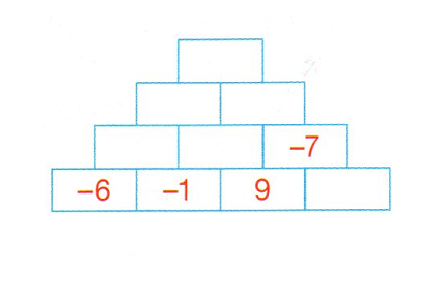
\includegraphics[scale=1]{pyramide.eps} \\
\end{center}



\exo{4} Calculer astucieusement les expressions suivantes \textbf{en détaillant vos étapes de calcul}.

\bmul{2} 

$A = -3+(+7)-(-3)+8-5+10$\\
\reponse[4]\\

 \columnbreak
 

$B = 135+(-154)-(-65)-46$\\
\reponse[4]\\


\emul

\newpage

\vspace*{0.2cm}

\bmul{2}

$M = 1,98+(-5,2)-(-3,4)+0,02-4,5$\\
\reponse[4]\\

\columnbreak

$R = 21-(-5+3)+(4-8)-21$\\
\reponse[4]\\

\emul

\exo{1.5} 

\bmul{2}
Des enfants lancent 4 fléchettes sur la cible représentée ci-contre.\\
On obtient :\\
\bi
\item 5 points pour un tir dans le rouge,
\item 2,5 points pour un tir dans le vert,
\item -1,75 point pour un tir dans le bleu,
\item -8 points si on rate la cible.
\ei

\columnbreak

\begin{center}
 
\includegraphics[scale=1]{cible.eps}
 \end{center} 
\emul

Voici les résultats des 4 compétiteurs :
\bmul{2}
\noindent Anaïs : rouge, vert, vert, raté\\
David : rouge, vert, bleu, raté

\columnbreak

\noindent Eva : rouge, raté, raté, rouge\\
Sacha : vert, vert, bleu, raté

\emul

$\rightarrow$ \textbf{Lequel de ces enfants a obtenu le meilleur score ? Justifier votre réponse.}\\
\reponse[5]\\

\vspace*{0.5cm}

\exo{+1} BONUS\\

\textbf{Trouve le bon chemin pour sortir du labyrinthe parallélépipédique ci-dessous.}

\bmul{2}

Tu peux te déplacer :\\

– soit horizontalement (sur le même étage), mais tu ne peux passer d'une case à l'autre que si les deux cases ont un côté commun et si le nombre de la case où tu vas est supérieur à celui de le case d'origine.\\

– soit verticalement (d'un étage à un autre), mais tu ne peux descendre que si la case du dessous contient un nombre inférieur à la case à celle du dessus.\\

\columnbreak

\begin{center}
 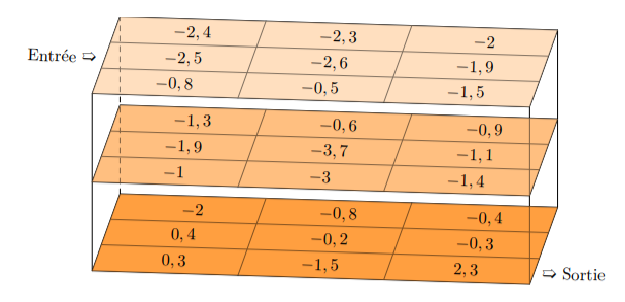
\includegraphics[scale=1]{bonus.eps}
 \end{center} 
 
 \emul


\end{document}
